%!TEX root = ./template-skripsi.tex

\subsection{Sprint 8 Report}
Berikut merupakan report dari sprint ke-8 yang dilakukan pada tanggal 13 juli - 19 juli 2022.

\begin{table}[H]
	\caption{\textit{Sprint-8 backlog}}
	\label{sprint8_backlog}
	\begin{tabular}{@{} |p{0.5cm}|p{5cm}|p{5cm}|p{2cm}| @{}}
		\hline
		\textbf{No} & \textbf{\textit{Story}} & \textbf{\textit{Task}} & \textbf{\textit{Status}} \\
		\hline
		1 & \multirow{3}{5cm}{Create, Read, Updte, dan Delete untuk Pencatatan grading berat ikan} & Membarui desain database  & Completed\\
		\cline{1-1}\cline{3-4}
		2 & & Menambahkan routes API & Completed\\
		\cline{1-1}\cline{3-4}
		3 & & Implementasi controller entry grading berat ikan & Completed\\
		\cline{1-1}\cline{3-4}
		4 & & Implementasi controller fetch list grading berat ikan & Completed\\
		\cline{1-1}\cline{3-4}
		5 & & Implementasi controller edit grading berat ikan & Completed\\
		\cline{1-1}\cline{3-4}
		6 & & Implementasi controller delete grading berat ikan & Completed\\
		\cline{1-1}\cline{3-4}
		7 & & Implementasi controller fetch grading berat ikan dengan id& Completed\\
		\cline{1-1}\cline{3-4}
		8 & & Membuat view rekap grading berat ikan & Completed\\
		\cline{1-1}\cline{3-4}
		\hline
	\end{tabular}
\end{table}

\begin{enumerate}[1.]

\item \textbf{Membarui desain database}

\begin{figure}[H]
	\centering
	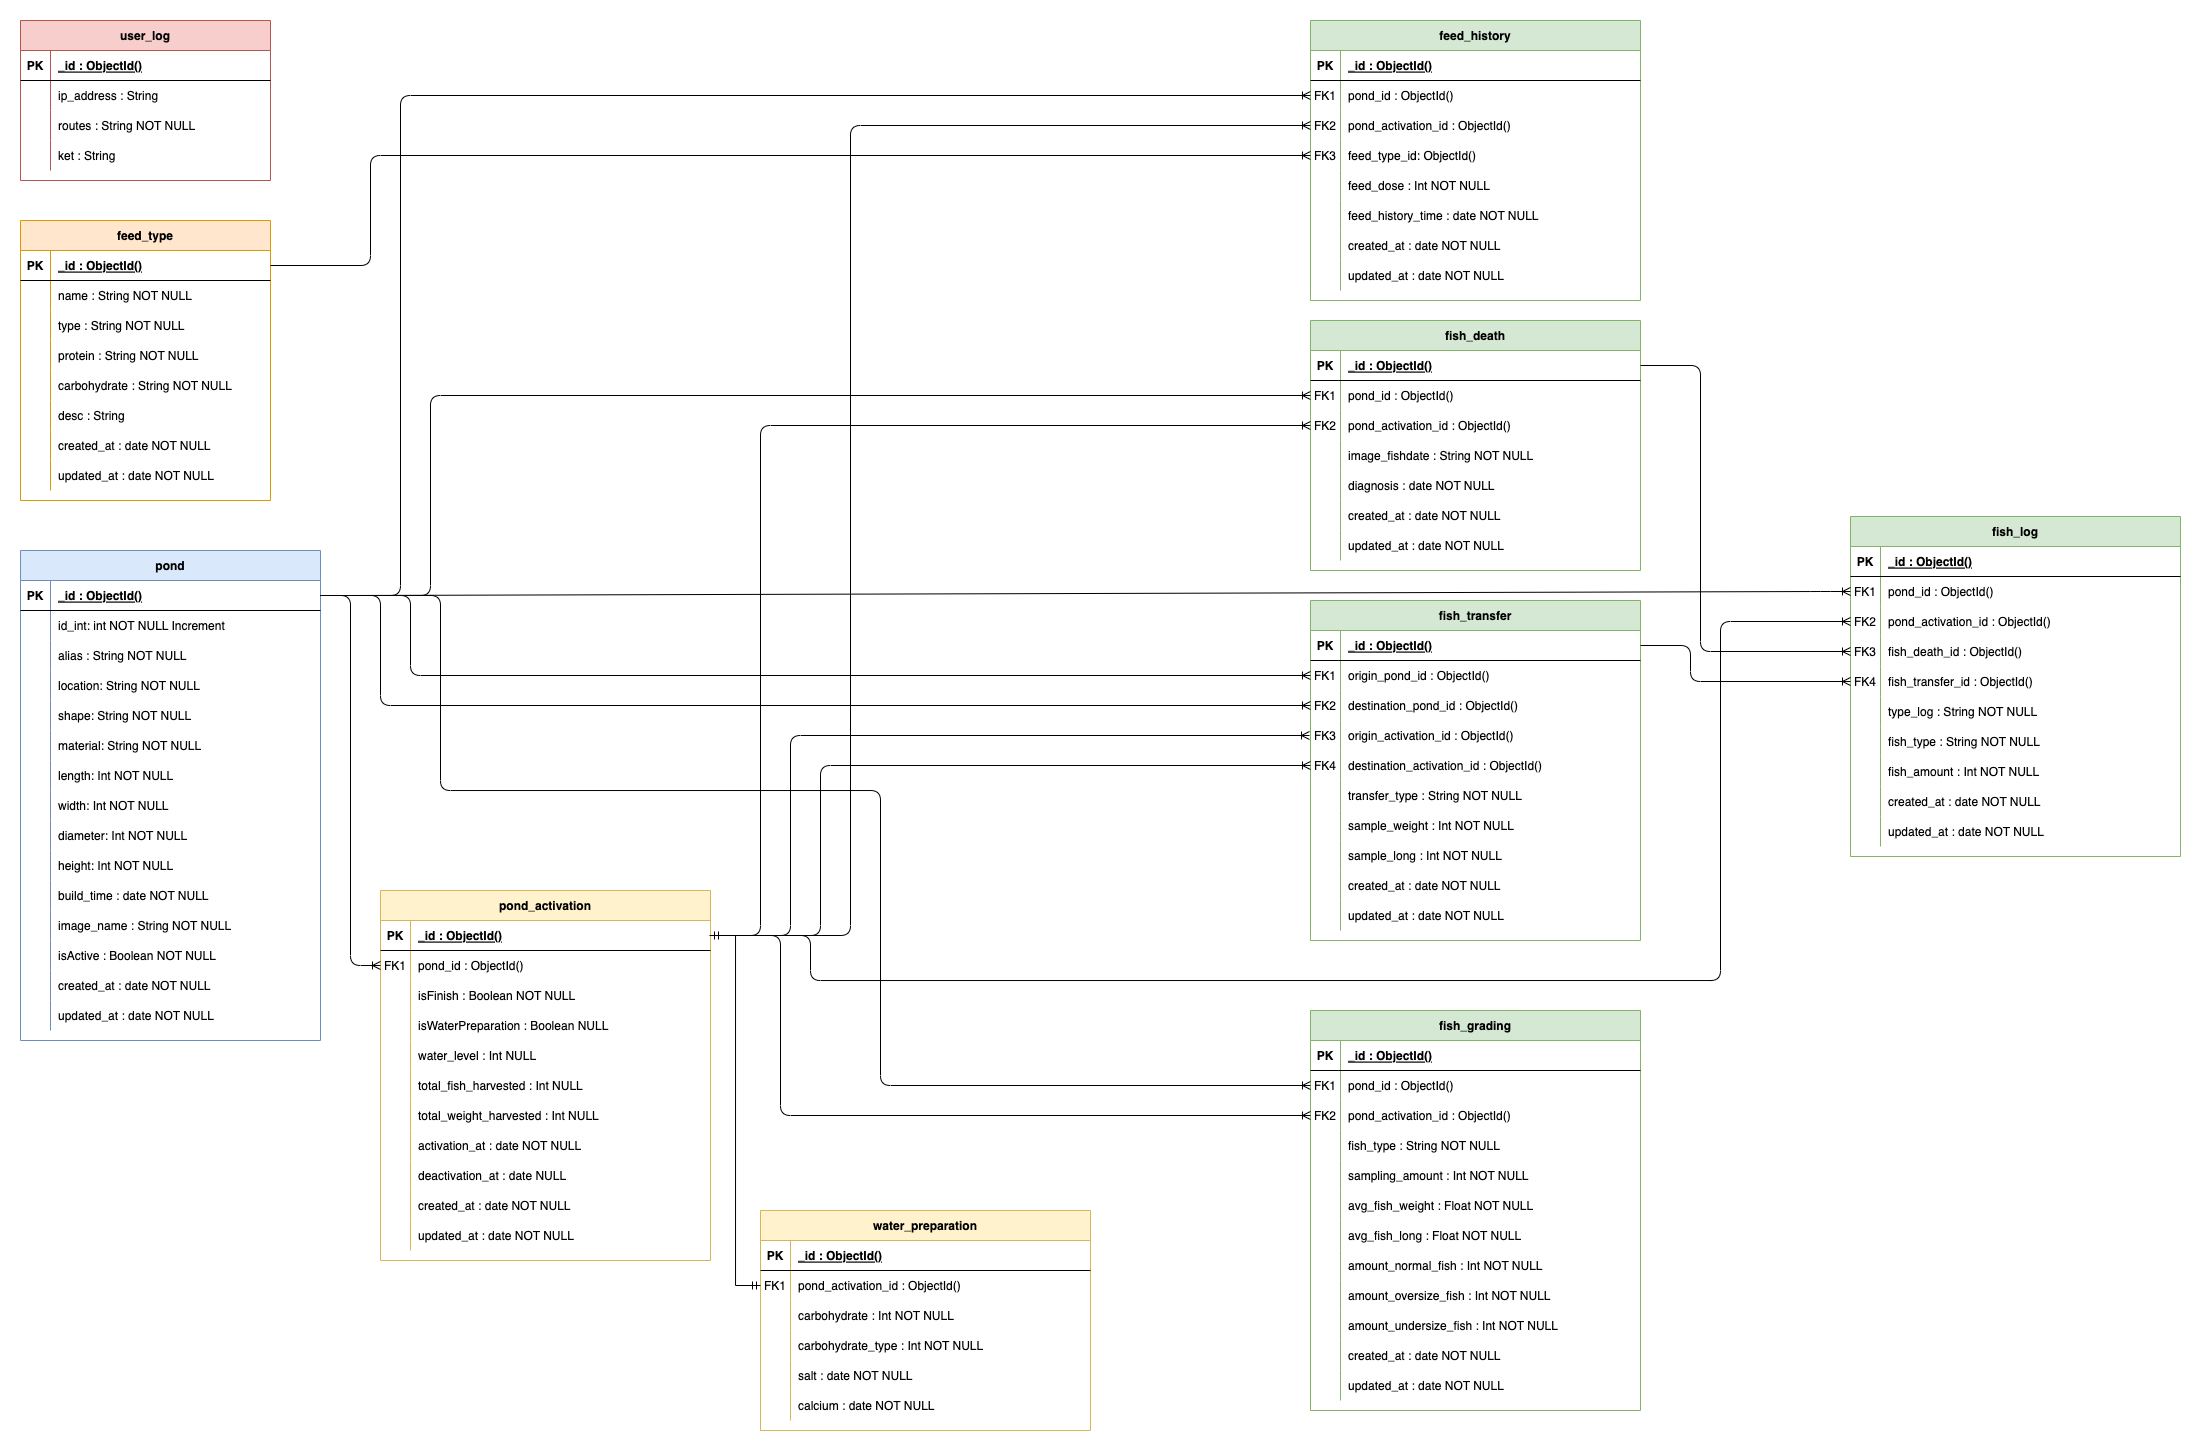
\includegraphics[height=0.7\textwidth]{gambar/Sprint08/diagram database/database}
	\caption{ERD Database Sprint-8}
	\label{fig:database_sprint8}
\end{figure}

Dengan berubahnya desain database diperlukan juga penambahan model pada source code, berikut perubahan pada source code model.

\begin{lstlisting}
# fishapi/database/model.py

class FishGrading(db.Document):
    pond_id = db.ReferenceField(Pond, required=True)
    pond_activation_id = db.ReferenceField(PondActivation, required=True)
    isOversizeTransferred = db.BooleanField(required=True, default=False)
    isUndersizeTransferred = db.BooleanField(required=True, default=False)
    fish_type = db.StringField(required=True)
    sampling_amount = db.IntField(required=True)
    avg_fish_weight = db.FloatField(required=True)
    avg_fish_long = db.FloatField(required=True)
    amount_normal_fish = db.IntField(required=True)
    amount_oversize_fish = db.IntField(required=True)
    amount_undersize_fish = db.IntField(required=True)
    grading_at = db.DateTimeField(default=datetime.datetime.now)
    created_at = db.DateTimeField(default=datetime.datetime.now)
    updated_at = db.DateTimeField(default=datetime.datetime.now)
\end{lstlisting}



\item \textbf{Menambahkan routes API}

\begin{lstlisting}
# fishapi/resource/routes.py

# fish grading
    api.add_resource(FishGradingsApi, '/api/fishgradings')
    api.add_resource(FishGradingApi, '/api/fishgradings/<id>')
    api.add_resource(FishGradingApiByActivation,
                     '/api/fishgradings/activation/<activation_id>')
    # graph
    api.add_resource(FishGradingGraphApi,
                     '/api/fishgradings/graph', endpoint='api.graph')
\end{lstlisting}




\item \textbf{Implementasi controller entry grading berat ikan}

Implementasi controller API entry grading berat ikan, berikut merupakan perubahan source code controller API entry grading berat ikan.

\begin{lstlisting}
# fishapi/resource/fishgrading.py

class FishGradingsApi(Resource):
    def post(self):
        try:
            pond_id = request.form.get("pond_id", None)
            pond = Pond.objects.get(id=pond_id)
            if pond['isActive'] == False:
                response = {"message": "pond is not active"}
                response = json.dumps(response, default=str)
                return Response(response, mimetype="application/json", status=400)
            pond_activation = PondActivation.objects(
                pond_id=pond_id, isFinish=False).order_by('-activated_at').first()
            body = {
                "pond_id": pond.id,
                "pond_activation_id": pond_activation.id,
                "fish_type": request.form.get("fish_type", None),
                "sampling_amount": request.form.get("sampling_amount", None),
                "avg_fish_weight": request.form.get("avg_fish_weight", None),
                "avg_fish_long": request.form.get("avg_fish_long", None),
                "amount_normal_fish": request.form.get("amount_normal_fish", None),
                "amount_oversize_fish": request.form.get("amount_oversize_fish", None),
                "amount_undersize_fish": request.form.get("amount_undersize_fish", None),
                "created_at": created_at,
                "grading_at": created_at,
            }
            fishgrading = FishGrading(**body).save()
            id = fishgrading.id
            return {'id': str(id)}, 200
        except Exception as e:
            response = {"message": str(e)}
            response = json.dumps(response, default=str)
            return Response(response, mimetype="application/json", status=400)
\end{lstlisting}

Kode di atas adalah sebuah API untuk mengelola data grading ikan. API ini menggunakan framework Flask-RESTful dan memiliki dua metode, yaitu get dan post.

Metode get digunakan untuk mendapatkan daftar grading ikan. Pada metode ini, digunakan agregasi MongoDB dengan pipeline untuk melakukan beberapa tahap pengolahan data. Pertama, terdapat dua tahap \$lookup yang digunakan untuk melakukan operasi join dengan koleksi "pond" dan "pond\_activation". Tahap-tahap ini mencocokkan nilai \_id dari transfer ikan dengan nilai dari field "pond\_id" dan "pond\_activation\_id" di koleksi yang di-lookup. Setelah itu, dengan menggunakan tahap \$addFields, ditambahkan dua field baru yaitu "pond" dan "pond\_activation" yang nilainya diambil dari hasil join sebelumnya menggunakan operator \$first. Tahap \$project digunakan untuk menghilangkan field "updated\_at" dan "created\_at" dari hasil akhir.

Setelah pipeline selesai, fungsi ini menggunakan metode aggregate() dari model FishGrading dengan menggunakan pipeline yang telah dibuat untuk mendapatkan hasilnya. Hasilnya kemudian dikonversi menjadi list dan disimpan dalam variabel list\_fishgradings.

Selanjutnya, hasil grading ikan tersebut diubah menjadi bentuk JSON menggunakan json.dumps(). JSON tersebut kemudian dikembalikan sebagai respons dengan tipe konten "application/json" dan kode status 200.

Jika terjadi kesalahan selama proses, pengecualian akan ditangkap dan sebuah respons JSON yang berisi pesan kesalahan akan dikirim. Pesan kesalahan akan menampilkan detail dari pengecualian yang terjadi. Respons JSON tersebut juga dikembalikan dengan tipe konten "application/json" dan kode status 400.

Metode post digunakan untuk membuat data grading ikan baru. Pada metode ini, terlebih dahulu dilakukan pengambilan nilai pond\_id dari form data yang dikirim. Kemudian, dilakukan pencarian kolam ("pond") berdasarkan pond\_id tersebut. Jika kolam tidak aktif (nilai "isActive" adalah False), maka dikembalikan respons JSON dengan pesan "pond is not active" dan kode status 400.

Selanjutnya, dilakukan pencarian aktivasi kolam ("pond\_activation") terbaru yang belum selesai (nilai "isFinish" adalah False) berdasarkan pond\_id. Nilai ini digunakan untuk mengisi field "pond\_activation\_id" pada data grading ikan yang akan dibuat.

Data grading ikan yang akan dibuat terdiri dari beberapa field yang diambil dari form data yang dikirim. Field "created\_at" dan "grading\_at" diisi dengan waktu saat ini. Data grading ikan tersebut kemudian disimpan ke dalam database menggunakan metode save().

Setelah data berhasil disimpan, ID dari data grading ikan yang baru dibuat diambil dan dikembalikan sebagai respons JSON dengan kode status 200.

Jika terjadi kesalahan selama proses, pengecualian akan ditangkap dan sebuah respons JSON yang berisi pesan kesalahan akan dikirim. Pesan kesalahan akan menampilkan detail dari pengecualian yang terjadi. Respons JSON tersebut juga dikembalikan dengan tipe konten "application/json" dan kode status 400.


Berikut merupakan form untuk entry grading berat ikan antar kolam.

\begin{longtable}{| l | p{5cm} | p{5cm} |}
\caption{Form entry kematian ikan.\label{table:form_entry_grading_berat_ikan}}\\

\hline
\multicolumn{1}{|c|}{\textbf{Form}} & \multicolumn{1}{|c|}{\textbf{Jenis Data}} & \multicolumn{1}{|c|}{\textbf{Deskripsi}}\\
\hline
\endfirsthead

\hline
\multicolumn{3}{|c|}{Lanjutan Tabel \ref{table:form_entry_grading_berat_ikan}}\\
\hline
\multicolumn{1}{|c|}{\textbf{Form}} & \multicolumn{1}{|c|}{\textbf{Jenis Data}} & \multicolumn{1}{|c|}{\textbf{Deskripsi}}\\
\hline
\endhead

                                          

pond\_id                & REQUIRED STRING                                                                & id kolam saat melakukan grading berat                                    \\ \hline
constanta\_oversize     & REQUIRED DOUBLE                                                                & konstanta yang menentukan berapa berat ikan yang dikategorikan oversize  \\ \hline
constanta\_undersize    & REQUIRED DOUBLE                                                                & konstanta yang menentukan berapa berat ikan yang dikategorikan undersize \\ \hline
fish\_type              & REQUIRED STRING TYPE; {[}"lele", "patin", "nila merah", "nila hitam", "mas"{]} & tipe ikan yang di grading beratnya                                       \\ \hline
sampling\_amount        & REQUIRED INT                                                                   & total jumlah ikan yang di lakukan sampling berat                         \\ \hline
avg\_fish\_weight       & REQUIRED DOUBLE                                                                & rata-rata berat ikan yang di sampling                                    \\ \hline
avg\_fish\_long         & REQUIRED DOUBLE                                                                & rata-rata panjang ikan yang di sampling                                  \\ \hline
amount\_normal\_fish    & REQUIRED INT                                                                   & jumlah ikan yang dikategorikan normal                                    \\ \hline
amount\_oversize\_fish  & REQUIRED INT                                                                   & jumlah ikan yang oversize                                                \\ \hline
amount\_undersize\_fish & REQUIRED INT                                                                   & jumlah ikan yang undersize                                               \\ \hline
\end{longtable}


Tabel di atas merupakan deskripsi dari kolom-kolom yang digunakan dalam suatu entitas data grading ikan. Tabel ini menjelaskan setiap kolom beserta tipe datanya dan penjelasan singkat tentang fungsinya.

Kolom pertama adalah "pond\_id" yang merupakan kolom wajib dengan tipe data STRING. Kolom ini digunakan untuk menyimpan ID kolam tempat dilakukannya grading berat pada ikan.

Kolom kedua dan ketiga adalah "constanta\_oversize" dan "constanta\_undersize" yang merupakan kolom wajib dengan tipe data DOUBLE. Kedua kolom ini digunakan untuk menyimpan konstanta yang menentukan batas berat ikan yang dikategorikan sebagai oversize atau undersize.

Kolom berikutnya adalah "fish\_type" yang merupakan kolom wajib dengan tipe data STRING. Kolom ini digunakan untuk menyimpan tipe ikan yang sedang dilakukan grading berat.

Selanjutnya, terdapat kolom "sampling\_amount" yang merupakan kolom wajib dengan tipe data INT. Kolom ini digunakan untuk menyimpan total jumlah ikan yang dilakukan sampling berat.

Kolom "avg\_fish\_weight" dan "avg\_fish\_long" adalah kolom wajib dengan tipe data DOUBLE. Kolom-kolom ini digunakan untuk menyimpan rata-rata berat dan panjang ikan yang diambil sebagai sampel.

Kolom "amount\_normal\_fish", "amount\_oversize\_fish", dan "amount\_undersize\_fish" adalah kolom wajib dengan tipe data INT. Kolom-kolom ini digunakan untuk menyimpan jumlah ikan yang dikategorikan sebagai normal, oversize, dan undersize, sesuai dengan hasil grading berat yang dilakukan.


Berikut merupakan hasil test request dari API entry perpindahan ikan antar kolam.

cURL:

\begin{lstlisting}
curl --location 'http://jft.web.id/fishapi/api/fishgradings' \
--form 'pond_id="{pond_id}"' \
--form 'fish_type="lele"' \
--form 'sampling_amount="20"' \
--form 'avg_fish_weight="50"' \
--form 'avg_fish_long="10"' \
--form 'amount_normal_fish="18"' \
--form 'amount_oversize_fish="1"' \
--form 'amount_undersize_fish="1"'
\end{lstlisting}

response json:

\begin{lstlisting}
{
  "message": "success add fish grading",
  "id": "62e105707ac8f837667faa70"
}
\end{lstlisting}




\item \textbf{Implementasi API fetch list grading berat ikan}

Implementasi controller API fetch list grading berat ikan, berikut merupakan source code controller API fetch list grading berat ikan.

\begin{lstlisting}
# fishapi/resource/fishgrading.py

def get(self):
        try:
            pipeline = [
                {'$lookup': {
                    'from': 'pond',
                    'let': {"pondid": "$pond_id"},
                    'pipeline': [
                        {'$match': {'$expr': {'$eq': ['$_id', '$$pondid']}}},
                        {"$project": {
                            "_id": 1,
                            "alias": 1,
                            "location": 1,
                            "build_at": 1,
                            "isActive": 1,
                        }}
                    ],
                    'as': 'pond'
                }},
                {'$lookup': {
                    'from': 'pond_activation',
                    'let': {"activationid": "$pond_activation_id"},
                    'pipeline': [
                        {'$match': {
                            '$expr': {'$eq': ['$_id', '$$activationid']}}},
                        {"$project": {
                            "_id": 1,
                            "isFinish": 1,
                            "isWaterPreparation": 1,
                            "water_level": 1,
                            "activated_at": 1
                        }}
                    ],
                    'as': 'pond_activation'
                }},
                {"$addFields": {
                    "pond": {"$first": "$pond"},
                    "pond_activation": {"$first": "$pond_activation"},
                }},
                {"$project": {
                    "updated_at": 0,
                    "created_at": 0,
                }}
            ]
            fishgrading = FishGrading.objects.aggregate(pipeline)
            list_fishgradings = list(fishgrading)
            response = json.dumps(list_fishgradings, default=str)
            return Response(response, mimetype="application/json", status=200)
        except Exception as e:
            response = {"message": str(e)}
            response = json.dumps(response, default=str)
            return Response(response, mimetype="application/json", status=400)
\end{lstlisting}



Kode di atas merupakan implementasi dari metode get dalam suatu API. Kode ini bertujuan untuk mengambil data grading ikan dari sumber data yang terhubung dan mengembalikan respons dalam format JSON.

Pada awalnya, kode ini mendefinisikan sebuah pipeline yang akan digunakan untuk melakukan operasi agregasi pada objek FishGrading. Pipeline ini terdiri dari beberapa tahap yang dijalankan secara berurutan. Tahap pertama menggunakan operasi \$lookup untuk melakukan join dengan koleksi "pond" berdasarkan kolom "pond\_id". Hasil join ini disimpan dalam field "pond".

Selanjutnya, terdapat tahap kedua yang juga menggunakan operasi \$lookup. Tahap ini melakukan join dengan koleksi "pond\_activation" berdasarkan kolom "pond\_activation\_id". Hasil join ini disimpan dalam field "pond\_activation".

Setelah itu, menggunakan tahap "\$addFields", nilai field "pond" dan "pond\_activation" diubah menjadi hanya menyimpan dokumen pertama dari hasil join, dengan menggunakan operasi \$first.

Tahap terakhir menggunakan operasi "\$project" untuk menghilangkan field "updated\_at" dan "created\_at" dari hasil akhir.

Setelah pipeline selesai, kode melakukan agregasi pada objek FishGrading dengan menggunakan pipeline yang telah dibuat. Hasil agregasi ini kemudian diubah menjadi list dan dikonversi menjadi JSON menggunakan json.dumps.

Jika tidak terjadi exception selama proses ini, respons berisi data grading ikan dalam format JSON dikembalikan dengan status 200. Namun, jika terjadi exception, sebuah pesan error dikirimkan dalam format JSON dengan status 400.

Berikut merupakan hasil test request dari API fetch list perpindahan ikan antar kolam.

cURL:

\begin{lstlisting}
curl --location 'http://jft.web.id/fishapi/api/fishgradings'
\end{lstlisting}

response json:

\begin{lstlisting}
[
  {
    "_id": "62e105307ac8f837667faa6f",
    "pond_id": "62a62163e445ffb9c5f746f3",
    "pond_activation_id": "62d3f2180d7265ab60f9cb83",
    "fish_type": "lele",
    "sampling_amount": 10,
    "avg_fish_weight": 50,
    "avg_fish_long": 10,
    "amount_normal_fish": 8,
    "amount_oversize_fish": 1,
    "amount_undersize_fish": 1,
    "pond": {
      "_id": "62a62163e445ffb9c5f746f3",
      "alias": "charlie",
      "location": "blok 2",
      "build_at": "2022-06-13 00:24:51.473000",
      "isActive": true
    },
    "pond_activation": {
      "_id": "62d3f2180d7265ab60f9cb83",
      "isFinish": false,
      "isWaterPreparation": true,
      "water_level": 100,
      "activated_at": "2022-07-17 18:27:20.511000"
    }
  },
  {
    "_id": "62e105707ac8f837667faa70",
    "pond_id": "62a62163e445ffb9c5f746f3",
    "pond_activation_id": "62d3f2180d7265ab60f9cb83",
    "fish_type": "lele",
    "sampling_amount": 20,
    "avg_fish_weight": 50,
    "avg_fish_long": 10,
    "amount_normal_fish": 18,
    "amount_oversize_fish": 1,
    "amount_undersize_fish": 1,
    "pond": {
      "_id": "62a62163e445ffb9c5f746f3",
      "alias": "charlie",
      "location": "blok 2",
      "build_at": "2022-06-13 00:24:51.473000",
      "isActive": true
    },
    "pond_activation": {
      "_id": "62d3f2180d7265ab60f9cb83",
      "isFinish": false,
      "isWaterPreparation": true,
      "water_level": 100,
      "activated_at": "2022-07-17 18:27:20.511000"
    }
  }
]
\end{lstlisting}



\item \textbf{Implementasi API edit grading berat ikan}

Implementasi controller API edit grading berat ikan, berikut merupakan perubahan source code controller API edit grading berat ikan.

\begin{lstlisting}
# fishapi/database/fishgrading.py

def put(self, id):
        try:
            body = request.form.to_dict(flat=True)
            FishGrading.objects.get(id=id).update(**body)
            response = {
                "message": "success change data fish grading", "id": id}
            response = json.dumps(response, default=str)
            return Response(response, mimetype="application/json", status=200)
        except Exception as e:
            response = {"message": str(e)}
            response = json.dumps(response, default=str)
            return Response(response, mimetype="application/json", status=400)
\end{lstlisting}

Kode yang diberikan merupakan implementasi metode put dalam suatu API. Tujuan dari kode ini adalah untuk memperbarui data grading ikan berdasarkan id yang diberikan.

Pertama, kode ini mengambil data dari permintaan (request) dalam format form dan mengubahnya menjadi dictionary menggunakan metode to\_dict(flat=True). Data tersebut akan disimpan dalam variabel body.

Selanjutnya, menggunakan metode get() dari model FishGrading, dilakukan pencarian data grading ikan berdasarkan id yang diberikan. Setelah data ditemukan, dilakukan pembaruan (update()) pada atribut-atribut data menggunakan nilai yang ada dalam body.

Apabila pembaruan berhasil dilakukan, kode akan mengembalikan respons yang berisi pesan sukses beserta id data yang telah diubah. Pesan dan respons tersebut akan diubah menjadi format JSON menggunakan json.dumps().

Namun, apabila terjadi kesalahan atau exception dalam proses pembaruan, kode akan menangkap exception tersebut dan mengembalikan respons yang berisi pesan error. Respons tersebut juga akan diubah menjadi format JSON sebelum dikirimkan kembali kepada pengguna.

Berikut merupakan hasil test request dari API edit grading berat ikan.

cURL:

\begin{lstlisting}
curl --location --request PUT 'http://jft.web.id/fishapi/api/fishgradings/62e105707ac8f837667faa70' \
--form 'fish_type="lele"' \
--form 'sampling_amount="21"' \
--form 'avg_fish_weight="50"' \
--form 'avg_fish_long="10"' \
--form 'amount_normal_fish="18"' \
--form 'amount_oversize_fish="2"' \
--form 'amount_undersize_fish="1"'
\end{lstlisting}

response json:

\begin{lstlisting}
{
  "message": "success change data fish grading",
  "id": "62e105707ac8f837667faa70"
}
\end{lstlisting}



\item \textbf{Implementasi API delete grading berat ikan}

Implementasi controller API delete grading berat ikan, berikut merupakan perubahan source code controller API delete grading berat ikan.

\begin{lstlisting}
# fishapi/database/fishgrading.py

def delete(self, id):
        try:
            fishgrading = FishGrading.objects.get(id=id).delete()
            response = {"message": "success delete fish grading"}
            response = json.dumps(response, default=str)
            return Response(response, mimetype="application/json", status=200)
        except Exception as e:
            response = {"message": str(e)}
            response = json.dumps(response, default=str)
            return Response(response, mimetype="application/json", status=400)
\end{lstlisting}

Tujuan dari kode ini adalah untuk menghapus data grading ikan berdasarkan id yang diberikan.

Pertama, menggunakan metode get() dari model FishGrading, dilakukan pencarian data grading ikan berdasarkan id yang diberikan. Setelah data ditemukan, metode delete() akan dipanggil untuk menghapus data tersebut.

Apabila penghapusan berhasil dilakukan, kode akan mengembalikan respons yang berisi pesan sukses untuk memberitahu bahwa data grading ikan telah berhasil dihapus.

Namun, jika terjadi kesalahan atau exception dalam proses penghapusan, kode akan menangkap exception tersebut dan mengembalikan respons yang berisi pesan error yang menjelaskan kesalahan yang terjadi.

Selanjutnya, respons tersebut akan diubah menjadi format JSON menggunakan json.dumps() sebelum dikirimkan kembali kepada pengguna melalui objek Response dengan jenis konten application/json dan status kode 200 untuk respons sukses, atau status kode 400 untuk respons yang mengindikasikan terjadinya kesalahan.

Berikut merupakan hasil test request dari API delete grading berat ikan.

cURL:

\begin{lstlisting}
curl --location --request DELETE 'http://jft.web.id/fishapi/api/fishgradings/62e10cda1370aa28b4905284'
\end{lstlisting}

response json:

\begin{lstlisting}
{
  "message": "success delete fish grading"
}
\end{lstlisting}


\item \textbf{Implementasi API fetch detail grading berat ikan}

Implementasi controller API fetch detail grading berat ikan, berikut merupakan source code controller API fetch detail grading berat ikan.

\begin{lstlisting}
# fishapi/resource/fishgrading.py

def get(self, id):
        try:
            pipeline = [
                {'$match': {'$expr': {'$eq': ['$_id', {'$toObjectId': id}]}}},
                {'$lookup': {
                    'from': 'pond',
                    'let': {"pondid": "$pond_id"},
                    'pipeline': [
                        {'$match': {'$expr': {'$eq': ['$_id', '$$pondid']}}},
                        {"$project": {
                            "_id": 1,
                            "alias": 1,
                            "location": 1,
                            "build_at": 1,
                            "isActive": 1,
                        }}
                    ],
                    'as': 'pond'
                }},
                {'$lookup': {
                    'from': 'pond_activation',
                    'let': {"activationid": "$pond_activation_id"},
                    'pipeline': [
                        {'$match': {
                            '$expr': {'$eq': ['$_id', '$$activationid']}}},
                        {"$project": {
                            "_id": 1,
                            "isFinish": 1,
                            "isWaterPreparation": 1,
                            "water_level": 1,
                            "activated_at": 1
                        }}
                    ],
                    'as': 'pond_activation'
                }},
                {"$addFields": {
                    "pond": {"$first": "$pond"},
                    "pond_activation": {"$first": "$pond_activation"},
                }},
                {"$project": {
                    "updated_at": 0,
                    "created_at": 0,
                }}
            ]
            fishgrading = FishGrading.objects.aggregate(pipeline)
            list_fishgradings = list(fishgrading)
            response = json.dumps(list_fishgradings[0], default=str)
            return Response(response, mimetype="application/json", status=200)
        except Exception as e:
            response = {"message": str(e)}
            response = json.dumps(response, default=str)
            return Response(response, mimetype="application/json", status=400)
\end{lstlisting}


Kode di atas merupakan implementasi metode get dalam suatu API yang digunakan untuk mendapatkan data grading ikan berdasarkan id yang diberikan.

Pada awalnya, kode tersebut membentuk sebuah pipeline yang berisi serangkaian operasi agregasi untuk mengambil data. Pertama, dilakukan pencocokan (\$match) dengan membandingkan \_id dengan id yang diterima setelah diubah menjadi objek ObjectId menggunakan \$toObjectId.

Selanjutnya, dilakukan operasi \$lookup dua kali untuk menggabungkan data dengan koleksi "pond" dan "pond\_activation" berdasarkan nilai yang sesuai. Dalam operasi \$lookup, variabel (let) digunakan untuk menyimpan nilai yang akan digunakan dalam pipeline yang sesuai. Setelah itu, dengan menggunakan \$project, hanya kolom-kolom tertentu yang dipilih untuk ditampilkan.

Kemudian, dengan menggunakan FishGrading.objects.aggregate(pipeline), pipeline akan dieksekusi dan menghasilkan objek agregat. Objek agregat tersebut kemudian dikonversi menjadi list menggunakan list(fishgrading). Dalam kasus ini, karena hanya ingin mengambil data pertama dari hasil tersebut, digunakan indeks [0] untuk mengakses elemen pertama dari list.

Hasil akhir dari elemen pertama tersebut kemudian diubah menjadi JSON menggunakan json.dumps, dan dikembalikan sebagai respons dengan tipe konten "application/json" dan status kode 200 jika berhasil. Jika terjadi kesalahan, tangkapan Exception akan menghasilkan pesan kesalahan yang dikirim sebagai respons dengan status kode 400.

Berikut merupakan hasil test request dari API fetch list grading berat ikan.

cURL:

\begin{lstlisting}
curl --location 'http://jft.web.id/fishapi/api/fishgradings/62e105707ac8f837667faa70'
\end{lstlisting}

response json:

\begin{lstlisting}
{
  "_id": "62e105707ac8f837667faa70",
  "pond_id": "62a62163e445ffb9c5f746f3",
  "pond_activation_id": "62d3f2180d7265ab60f9cb83",
  "fish_type": "lele",
  "sampling_amount": 20,
  "avg_fish_weight": 50,
  "avg_fish_long": 10,
  "amount_normal_fish": 18,
  "amount_oversize_fish": 1,
  "amount_undersize_fish": 1,
  "pond": {
    "_id": "62a62163e445ffb9c5f746f3",
    "alias": "charlie",
    "location": "blok 2",
    "build_at": "2022-06-13 00:24:51.473000",
    "isActive": true
  },
  "pond_activation": {
    "_id": "62d3f2180d7265ab60f9cb83",
    "isFinish": false,
    "isWaterPreparation": true,
    "water_level": 100,
    "activated_at": "2022-07-17 18:27:20.511000"
  }
}
\end{lstlisting}



\end{enumerate}